\normaltrue
\correctionfalse

%\UPSTIidClasse{11} % 11 sup, 12 spé
%\newcommand{\UPSTIidClasse}{12}

\exer{Cours de cinétique  $\star$ \label{DYN:04:cours}}
\setcounter{question}{0}\marginnote{\xpComp{DYN}{04}}%\xpComp{CIN}{02}%\UPSTIcompetence[2]{C2-05}


\index{Compétence DYN-04}

\ifcorrection
\else
\marginnote{\textbf{Pas de corrigé pour cet exercice.}}
\fi


\question{Donner l'expression du moment cinétique en un point quelconque.}
\ifprof~\\
\else
\fi

\question{Donner l'expression du moment dynamique en un point quelconque.}
\ifprof~\\
\else
\fi

\question{Donner l'expression du torseur cinétique. }
\ifprof~\\
\else
\fi

\question{Donner l'expression du torseur dynamique. }
\ifprof~\\
\else
\fi

\begin{marginfigure}
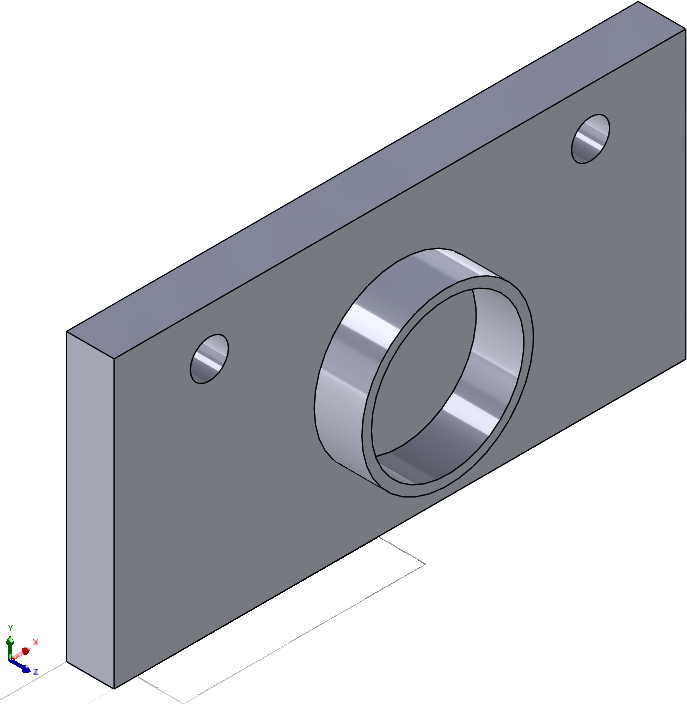
\includegraphics[width=\linewidth]{cours_01}
\end{marginfigure}
\question{Proposer une expression de la matrice d'inertie du solide au point de votre choix. }
\ifprof~\\
\else
\fi


\ifprof
\else
\marginnote{Corrigé  voir \ref{DYN:04:cours}.}
\fi